\section{Introduction}

Large Language Models (LLMs) power chatbots \citep{anthropic2023claude,openai2024gpt4technicalreport}, search engines \citep{google2023bard}, and coding assistants \citep{copilot}. Inference---generating responses to queries---imposes significant memory and compute demands \citep{garcia2019estimation}. Efficient scheduling is critical: ChatGPT incurs daily costs exceeding \$700,000 \citep{patel2023peeling}.

LLM inference (Figure~\ref{fig:intro_example}) proceeds in two phases. In the \textbf{prefill} phase, the model tokenizes input and builds a Key-Value (KV) cache storing attention keys and values. In the \textbf{decode} phase, output tokens are generated sequentially, with each step querying and updating the KV cache. KV cache memory grows linearly with output length, creating resource demands that change during processing.

\begin{figure}
    \centering
    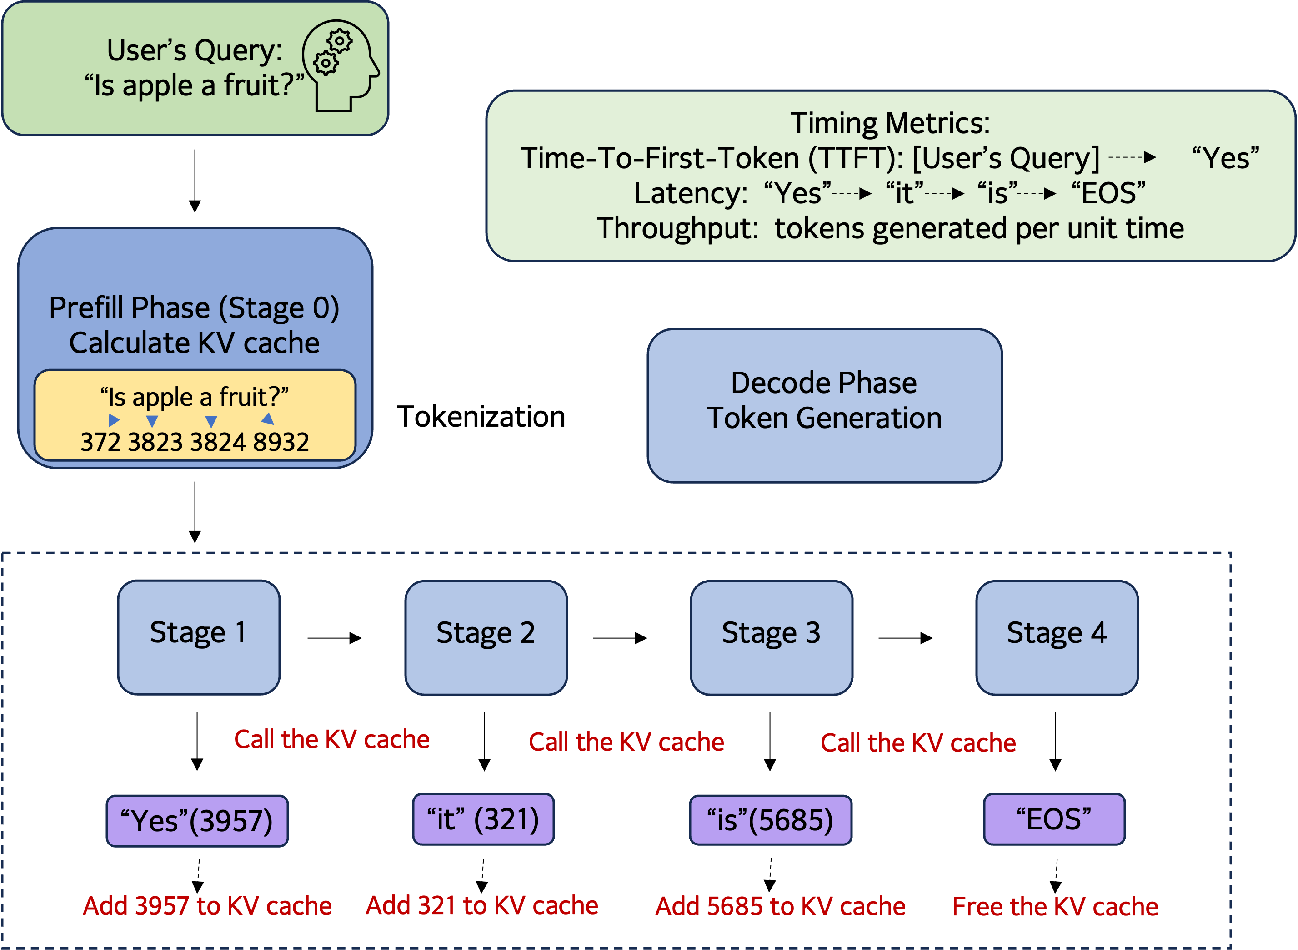
\includegraphics[width=0.6\linewidth]{Experiments_pdf/fig_intro.pdf}
    \caption{LLM inference service process.}
    \label{fig:intro_example}
\end{figure}

The KV cache avoids quadratic recomputation but creates capacity challenges: memory grows unpredictably, and exceeding GPU limits degrades performance \citep{kang2024gear}. Batching optimizes GPU use, but traditional scheduling (e.g., Shortest Job First) assumes fixed job sizes and known processing times—inapplicable when KV cache grows dynamically and output lengths are unknown. Classical OR approaches fail for this multi-phase, memory-constrained setting.

Recent system-level optimizations \citep{yu2022orca, kwon2023efficient, agrawal2023sarathi, pope2023efficiently, deepseekai2024deepseekv2strongeconomicalefficient, patel2024splitwise, zhong2024distserve} focus on engineering solutions but lack rigorous mathematical foundations. Output length predictions are imprecise or costly \citep{fu2025efficient}. When output lengths are unknown, algorithm performance degrades (Proposition \ref{prop:unknown_lower_bound}).

We develop a fluid dynamics approximation to establish a tractable benchmark. From this benchmark, we derive the WAIT algorithm for known output lengths and Nested WAIT for unknown lengths. Nested WAIT uses hierarchical thresholds to manage random arrivals without predicting service times; prompts classify themselves on-the-fly by completing or continuing at segment boundaries. Both algorithms achieve asymptotic near-optimality.

\subsection{Summary of Contributions}

We make three contributions. First, we formulate LLM inference as a multi-stage online scheduling problem under memory constraints (Section~\ref{sec:model}) and employ fluid dynamics to establish a tractable performance benchmark (Section~\ref{sec:fluid}). Second, we develop WAIT for known output lengths (Section~\ref{sec:wait}) and Nested WAIT for unknown lengths (Section~\ref{sec:nested_wait}), proving asymptotic optimality via coupling analyses; extensions appear in Section~\ref{sec:extension}. Third, experiments on LMSYS-Chat-1M with Llama2-7B demonstrate 12--25\% throughput improvement and 30\% latency reduction over vLLM \citep{kwon2023efficient} and Sarathi \citep{agrawal2023sarathi} (Section~\ref{sec:experiments}).

\subsection{Other Related Work}

\paragraph*{Online Scheduling and Queueing.}
Classical online scheduling \cite{devanur2009adwords,vee2010optimal,cole2014sample,balkanski2016power,lattanzi2020online,im2013online,lucier2013efficient,liu2015online,li2020online} and queueing theory use fluid models for near-optimal control \cite{mandelbaum1998strong,maglaras2000discrete,bauerle2002optimal,liu2011network}. However, LLM inference differs fundamentally: resource requirements grow dynamically (KV cache) and involve multi-phase processing (prefill/decode), unlike static single-phase jobs in classical scheduling.

\paragraph*{LLM Inference.}
Most LLM inference work focuses on system optimizations \cite{patel2023peeling,zhong2024distserve,yu2022orca,agrawal2023sarathi,agrawal2024taming,deepseekai2024deepseekv2strongeconomicalefficient,fu2025efficient} rather than theoretical analysis. Unknown output lengths cause significant performance degradation (Proposition \ref{prop:unknown_lower_bound}). We develop a scheduling framework using fluid dynamics and coupling techniques to achieve asymptotic optimality under unknown lengths. \cite{li2025throughput} propose a similar linear batch processing model achieving optimal throughput for work-conserving policies, but do not address KV cache memory management or latency metrics (TTFT, end-to-end latency) critical for interactive applications.


\subsection{Notations}
For integer $n\ge 1,$ we denote $[n]=\{1,2,\dots,n\}$ as the set of integers from $1$ to $n$. For $x\in\real$, denote $\lceil x\rceil$ as the smallest integer not smaller than $x$ and $\lfloor x\rfloor$ as the largest integer not greater than $x$. Denote $x_+=\max\{x, 0\}$. For set $S$, denote $|S|$ as its cardinality. For two functions $f(T)$ and $g(T)$, we use $f(T)=O(g(T))$ if there exists constant $c_1>0$ such that $f(T)\le c_1g(T)$ as $T\to+\infty$ and $f(T)=\Omega(g(T))$ if there exists constant $c_2>0$ such that $f(T)\ge c_2g(T)$ as $T\to +\infty$.
